\section{Exploratory Data Analysis}
\label{sec:datAnalisys}
What hypothesis tests and ad-hoc studies did you perform,
and how did you interpret the results of these? What patterns did you notice, and how
did you use these to make subsequent decisions?




\subsection{Data Analysis}

Different plots were created with the aim of understanding the behaviour of the different transportation systems. The following figures show some of the comparisons made, so far.

Figure \ref{fig:boxTrips} shows the boxplots of the monthly number of trips for the different transportation systems. Figure \ref{fig:a} for Uber's trips, Figure \ref{fig:b} for Yellow cab trips, Figure \ref{fig:c} for Green cab trips, and Figure \ref{fig:d} for MTA trips. The boxplots differentiate the trips between rush hours (orange boxes) and non-rush hours (blue boxes). From the figures, it can be seen that the MTA is busier in rush hours than in non-rush hours. Additionally, it is possible to see that there has been a significan increase of the number of trips taken by Uber from 2015 both in rush and non-rush hours; and a decrease on the number of trips taken by Yellow cabs, especially in rush hours. 

\begin{figure}%
\centering
\subfigure[Uber trips.]{%
\label{fig:a}%
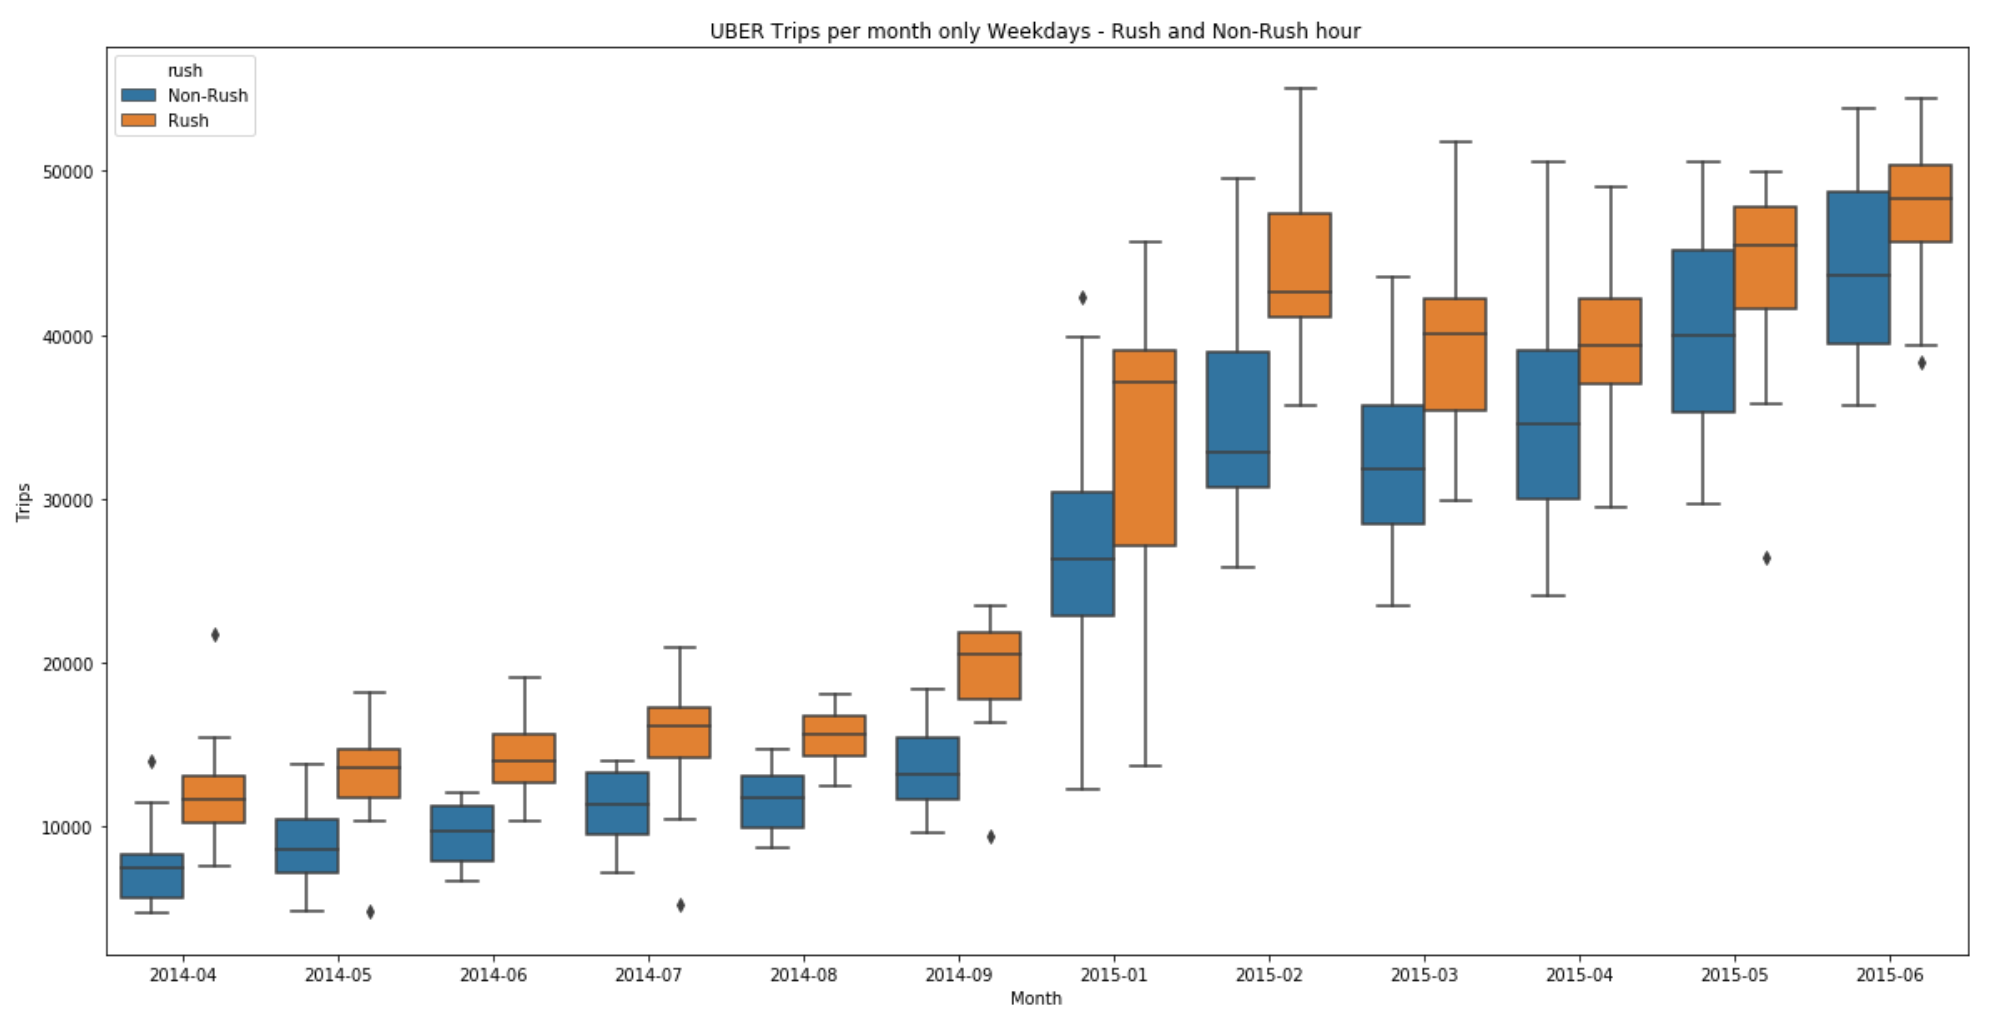
\includegraphics[height=2in, width=3.5in]{UBER_trips_only_weekdays_rush_and_non_rush.png}}%
\qquad
\subfigure[Yellow cab trips]{%
\label{fig:b}%
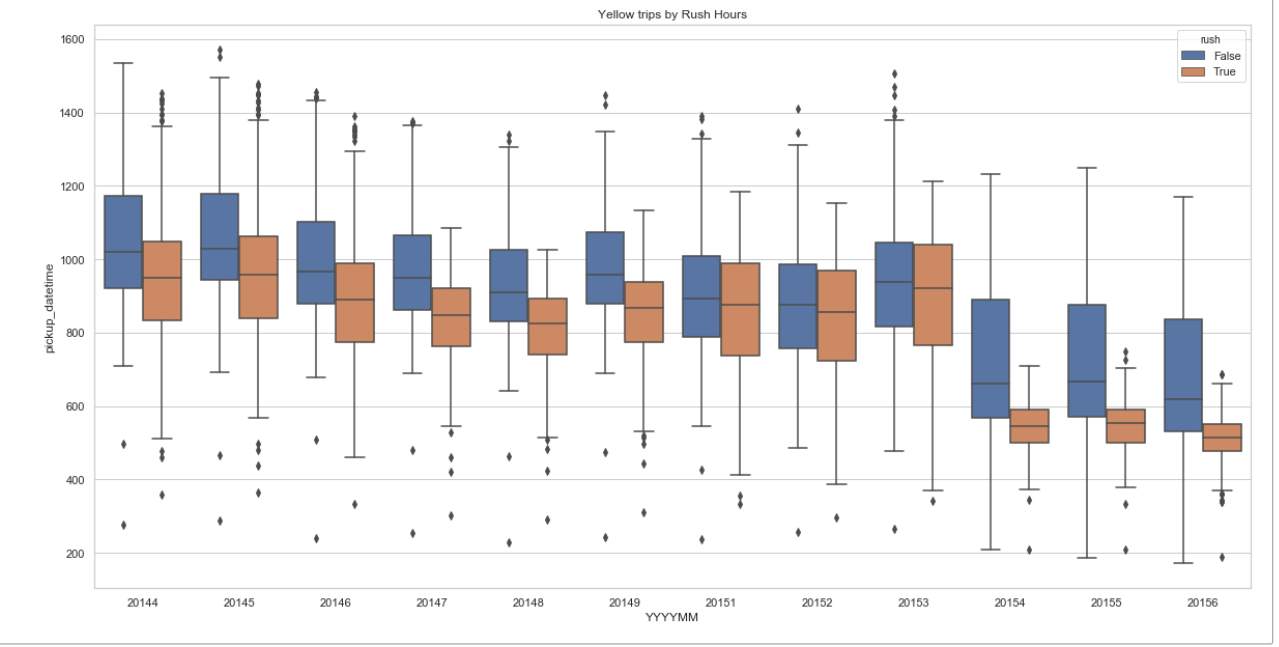
\includegraphics[height=2in, width=3.5in]{yellowTripsRushHours.png}}%
\qquad
\subfigure[Green cab trips]{%
\label{fig:c}%
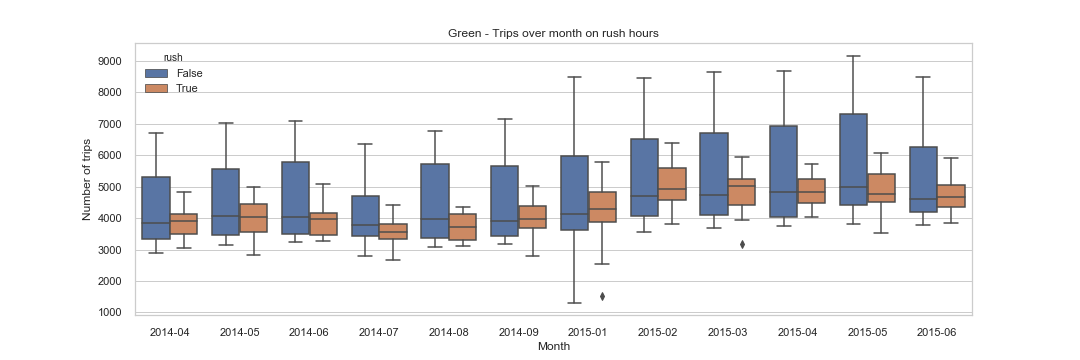
\includegraphics[height=2.4in, width=3.5in]{green_trips_month_rush.png}}%
\qquad
\subfigure[MTA trips]{%
\label{fig:d}%
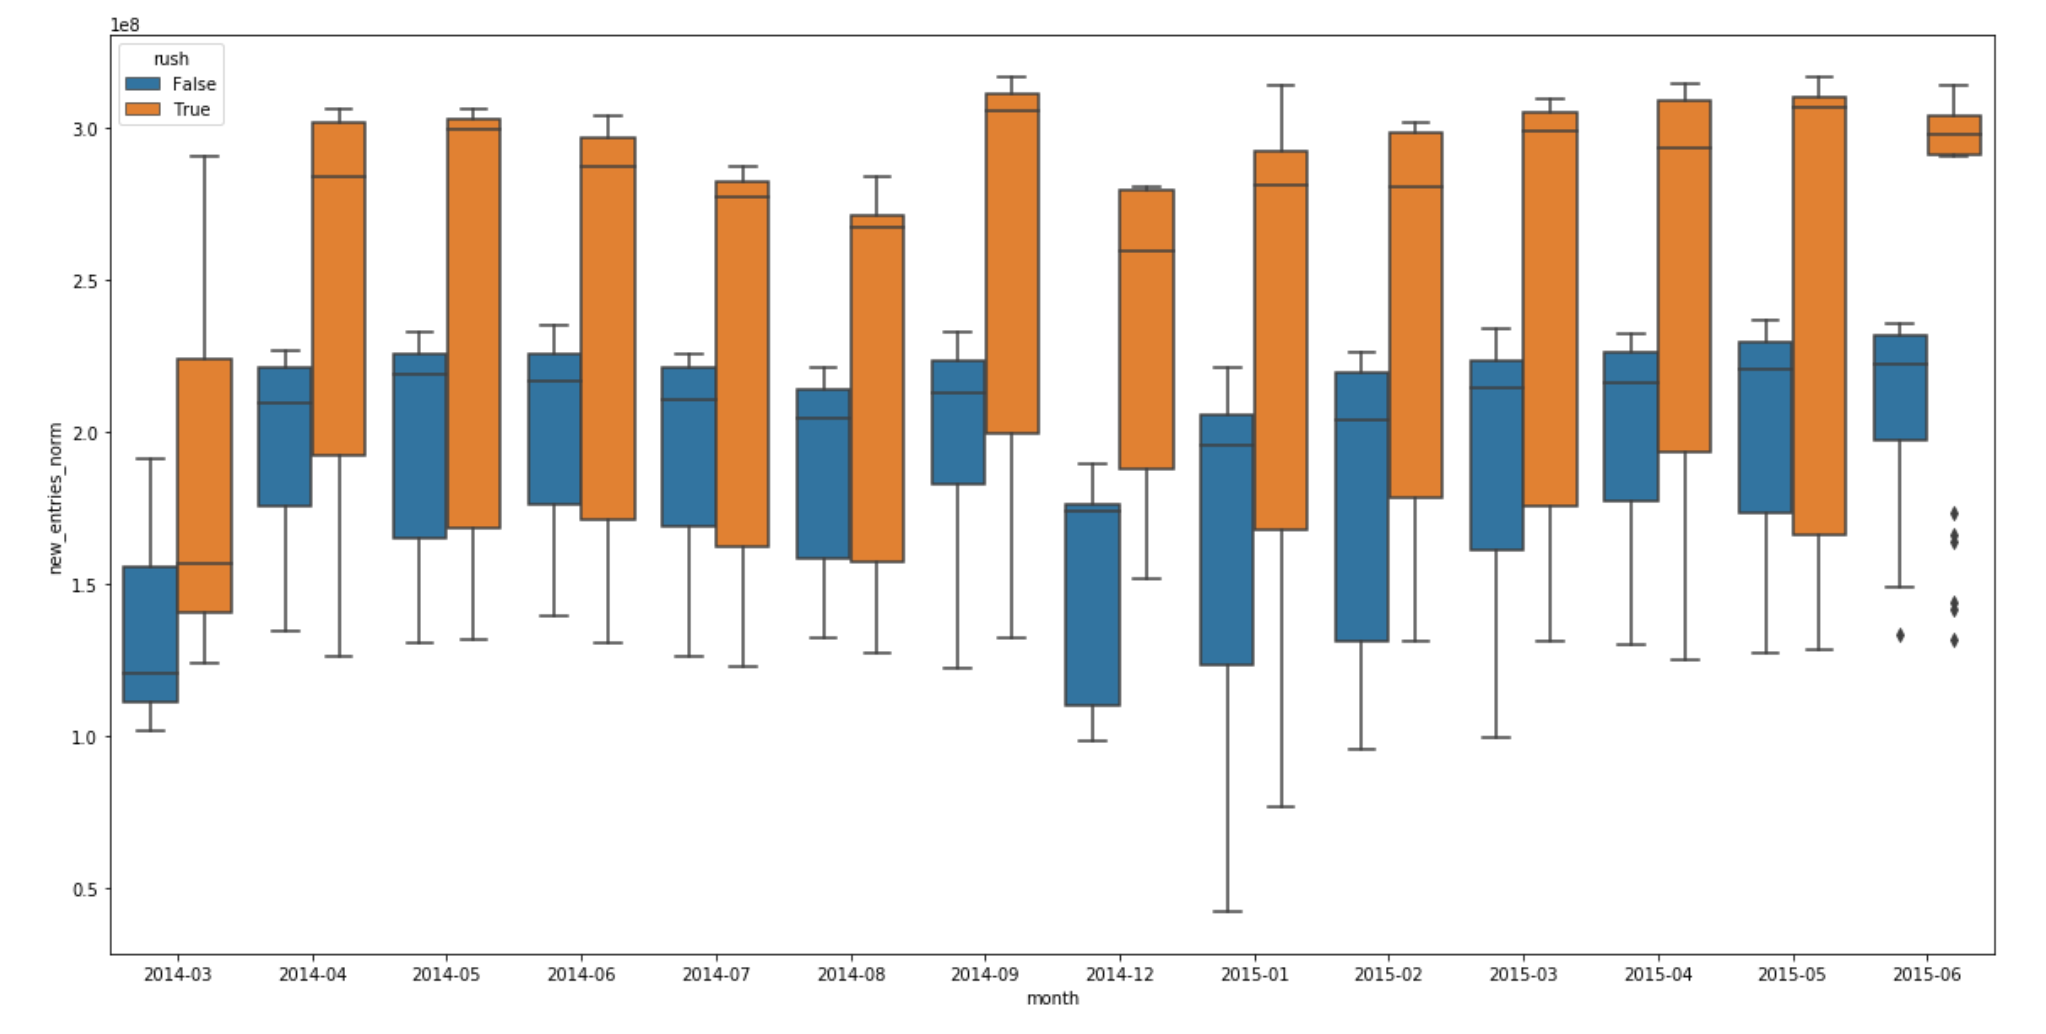
\includegraphics[height=2in, width=3.5in]{mta_new_entries_orange_rush_hour.png}}%
\caption{Has the increase of Uber trips affected the number of trips of Yellow cab, Green cab, and MTA trips? Orange boxes represent the number of trips in rush hours and blue ones correspond to non-rush hours. }
\label{fig:boxTrips}%
\end{figure}



Figure \ref{fig:boxDistances} compares the number of trips made by Uber with the monthly average travel distance covered by Yellow cabs. The aim of this comparison was to analyze if the increase of Uber trips affected the average travel distance of   plots, it is possible to see that from 2015, Uber is widely used for long distance trips, in contrast to Yellow cabs. On the other hand, the average travel distance of Yellow cabs experienced an increase in April 2015. 


\begin{figure}%
\centering
\subfigure[Uber]{%
\label{fig:first}%
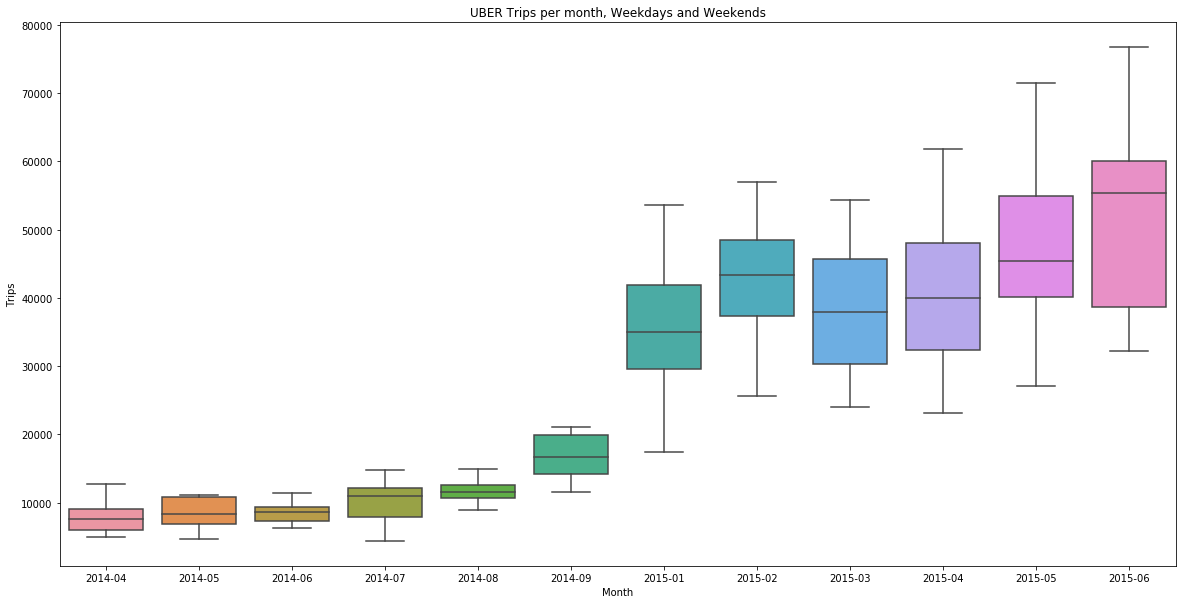
\includegraphics[height=2in, width=5in]{UBER_Trips_per_month_only_weekends.png}}%
\qquad
\subfigure[Yellow cabs]{%
\label{fig:second}%
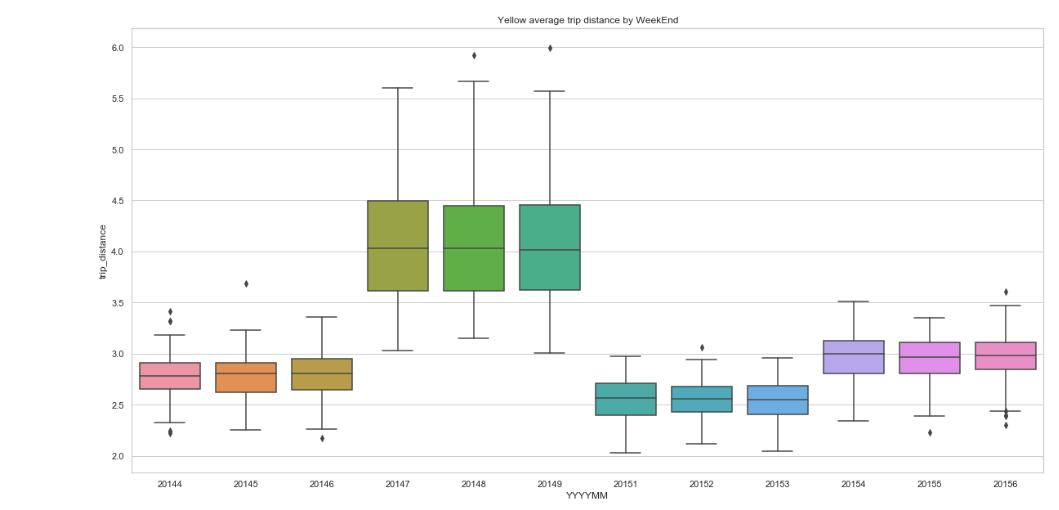
\includegraphics[height=2.2in, width=5.5in]{Yellow_Cabs_Average_trip_distance_Weekend_Only_by_Month_copy.png}}%
\caption{Has the increase of Uber trips affected the average travel distance of Yellow cab trips? Comparison of the monthly number of trips performed by Uber and the monthly average travel distance covered by Yellow cabs. Yellow }
\label{fig:boxDistances}%
\end{figure}




\begin{figure}%
\centering
\subfigure[Uber trips.]{%
\label{fig:a}%
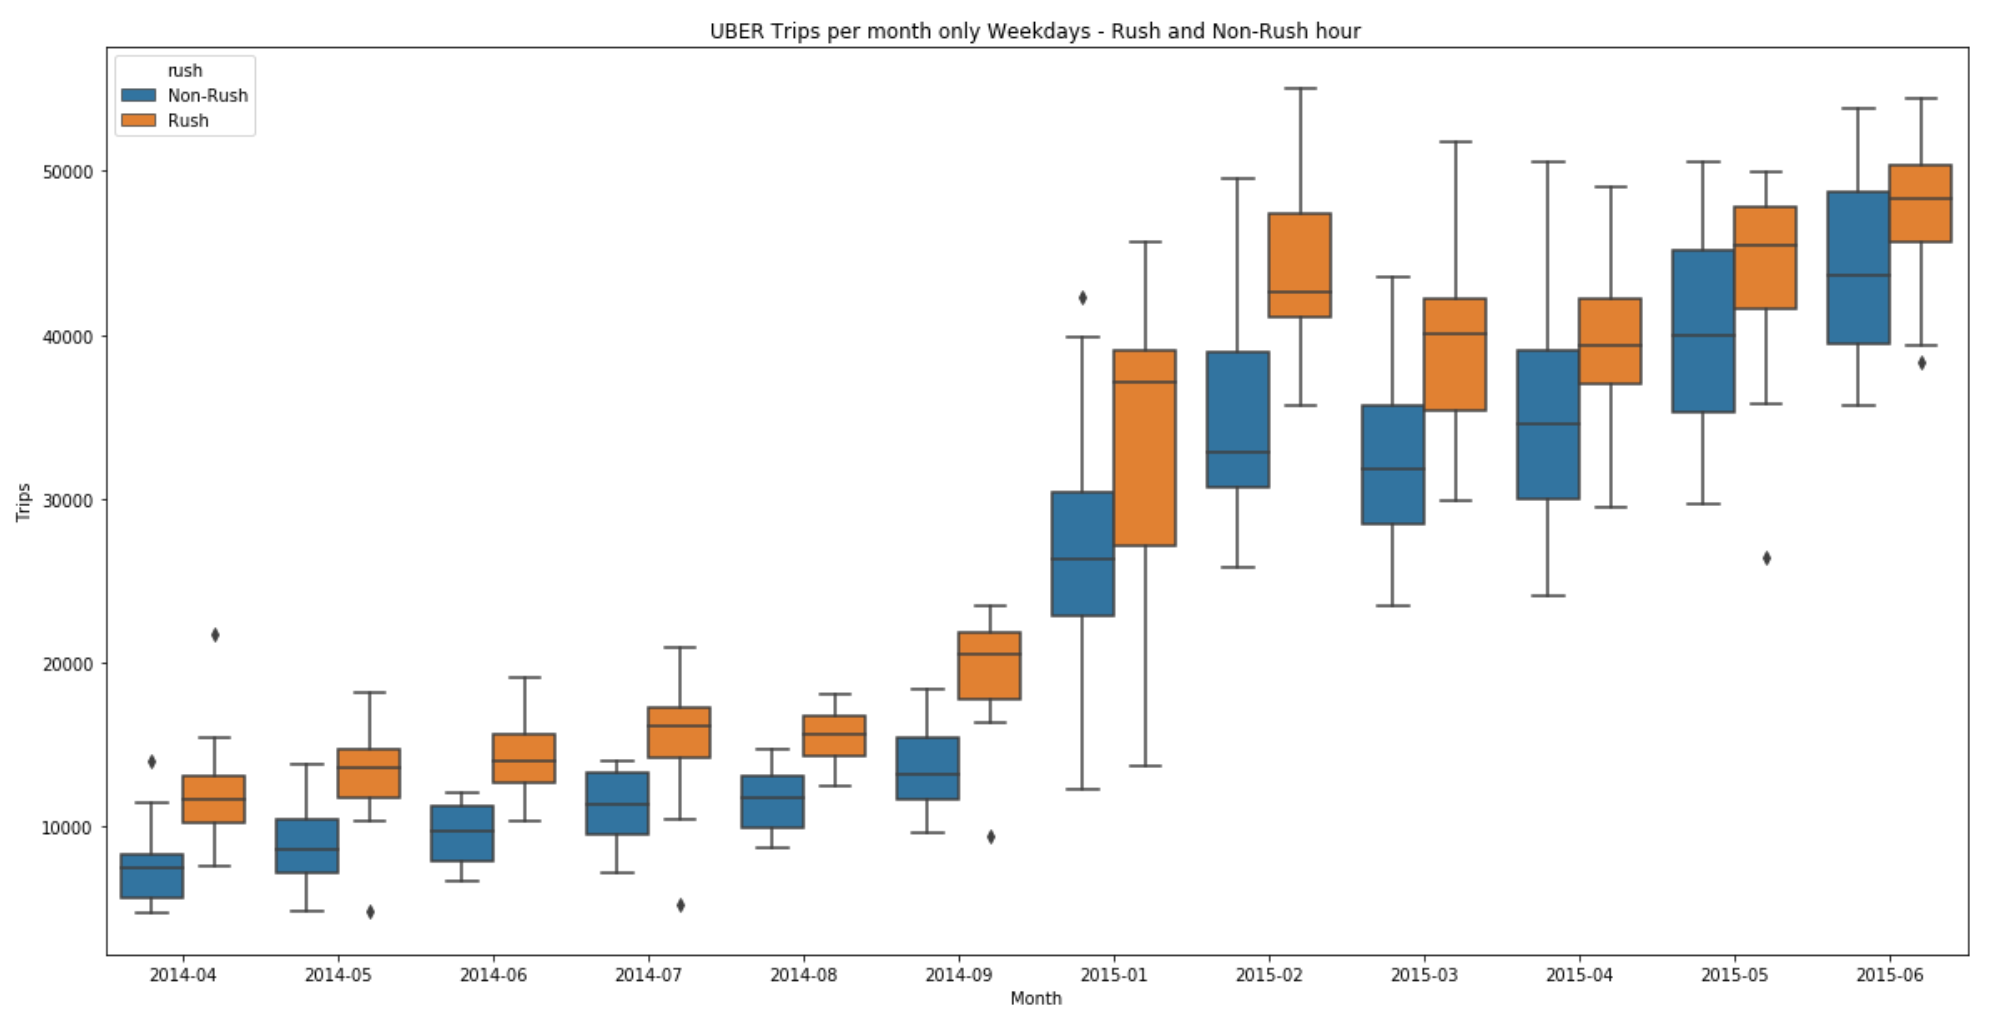
\includegraphics[height=2in, width=3.5in]{UBER_trips_only_weekdays_rush_and_non_rush.png}}%
\qquad
\subfigure[Yellow cab trips]{%
\label{fig:b}%
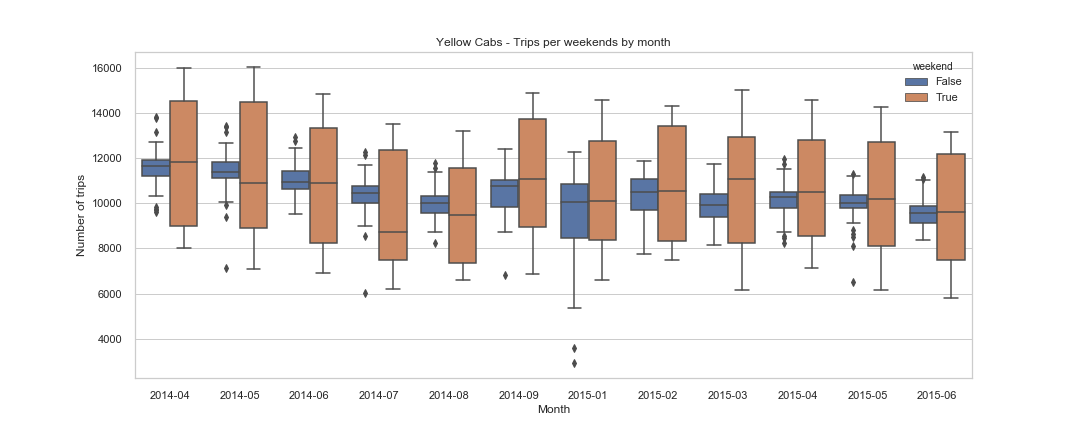
\includegraphics[height=2in, width=3.5in]{yellow_trips_month_weekend.png}}%
\qquad
\subfigure[Green cab trips]{%
\label{fig:c}%
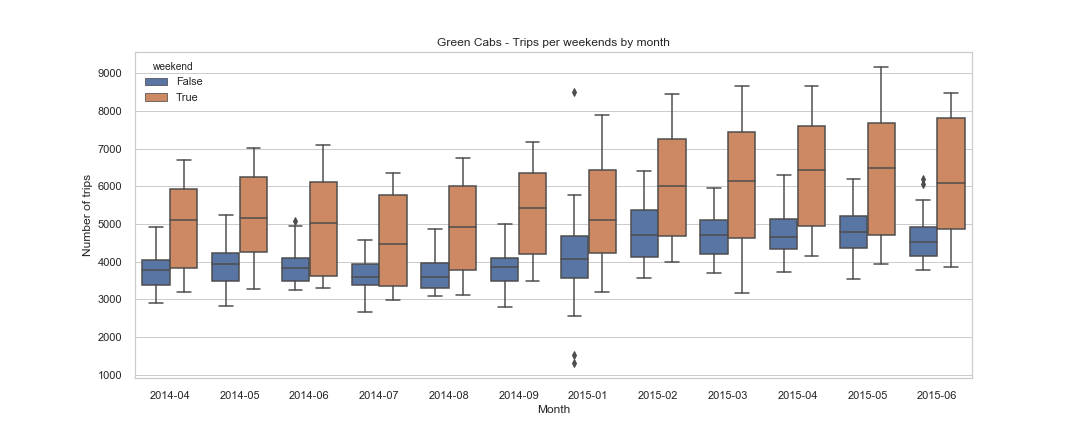
\includegraphics[height=2.4in, width=3.5in]{green_trips_month_weekend.png}}%
\qquad
\subfigure[MTA trips]{%
\label{fig:d}%
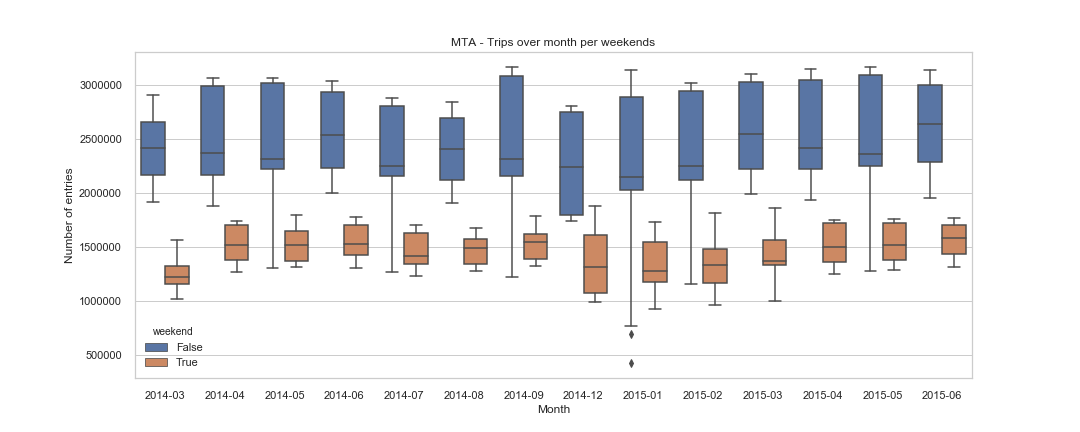
\includegraphics[height=2in, width=3.5in]{mta_entries_month_weekend.png}}%
\caption{trips weekend by month }
\label{fig:boxTrips}%
\end{figure}




\begin{figure}%
\centering
\subfigure[Uber trips.]{%
\label{fig:a}%
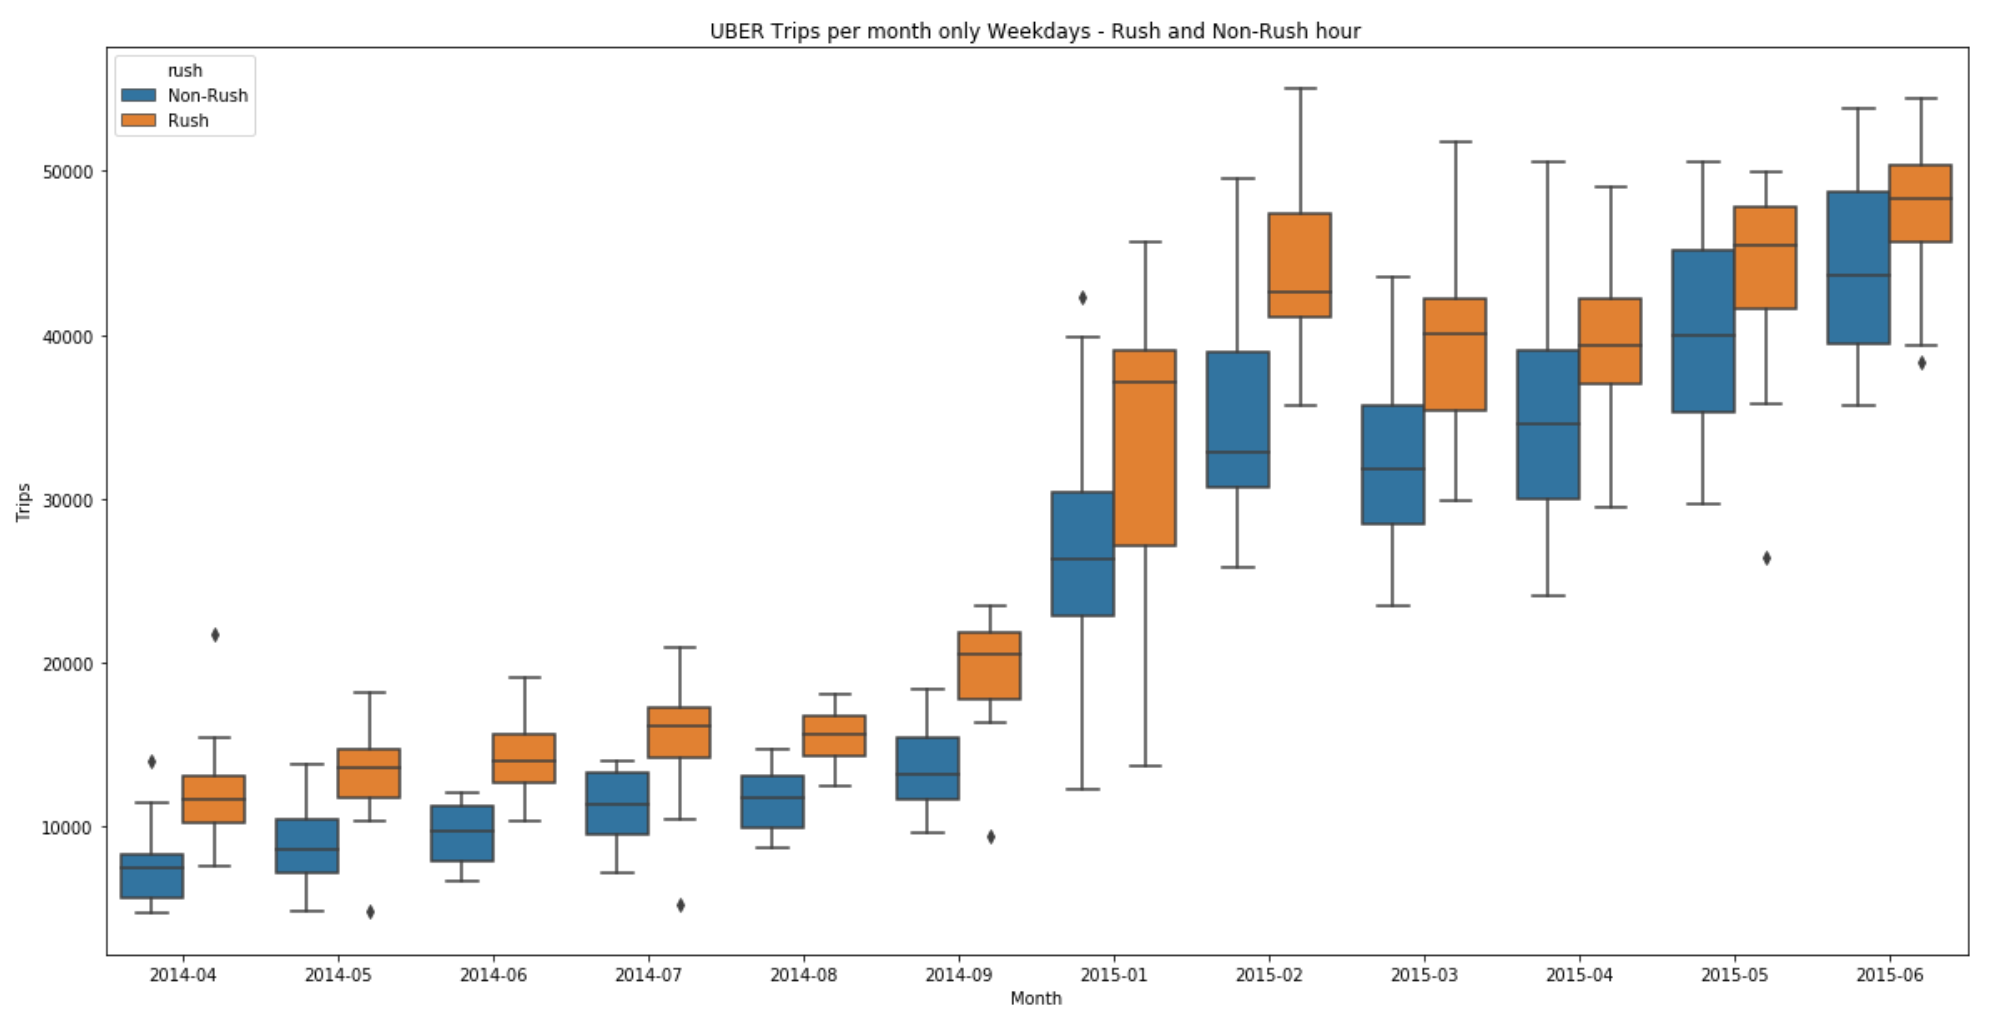
\includegraphics[height=2in, width=3.5in]{UBER_trips_only_weekdays_rush_and_non_rush.png}}%
\qquad
\subfigure[Yellow cab trips]{%
\label{fig:b}%
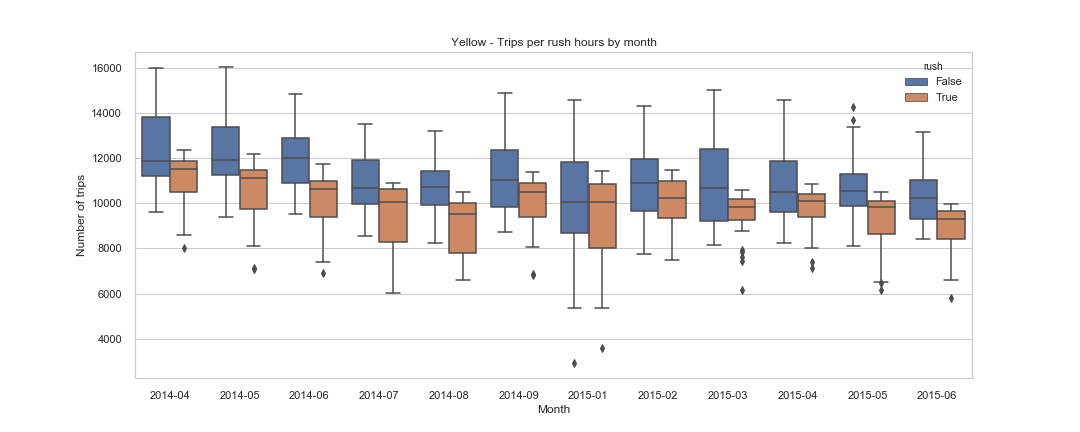
\includegraphics[height=2in, width=3.5in]{yellow_trips_month_rush.png}}%
\qquad
\subfigure[Green cab trips]{%
\label{fig:c}%
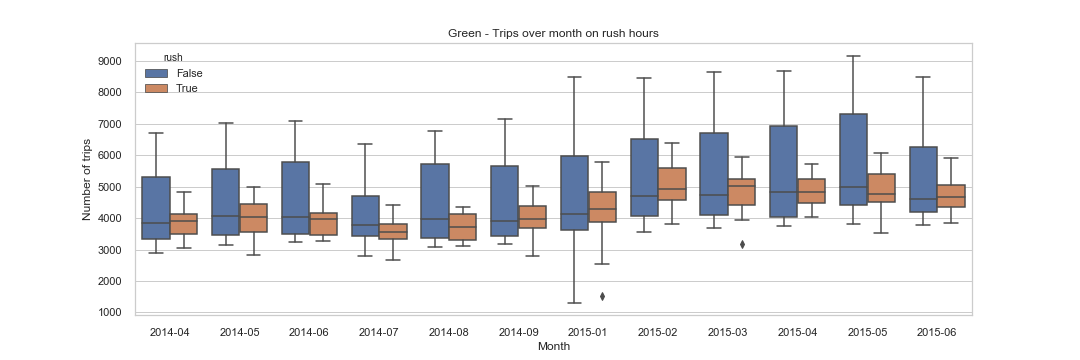
\includegraphics[height=2.4in, width=3.5in]{green_trips_month_rush.png}}%
\qquad
\subfigure[MTA trips]{%
\label{fig:d}%
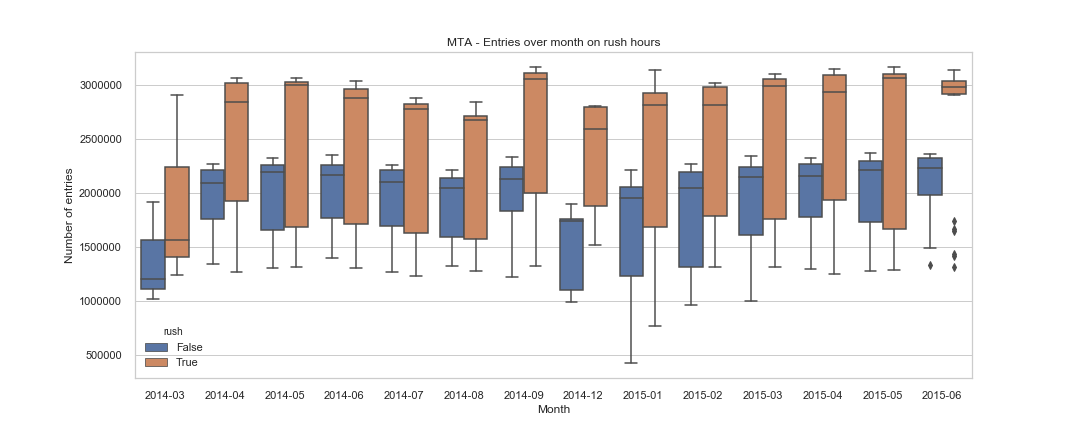
\includegraphics[height=2in, width=3.5in]{mta_entries_month_rush.png}}%
\caption{trips month rush hours }
\label{fig:boxTrips}%
\end{figure}




\begin{figure}%
\centering
\subfigure[Uber trips.]{%
\label{fig:a}%
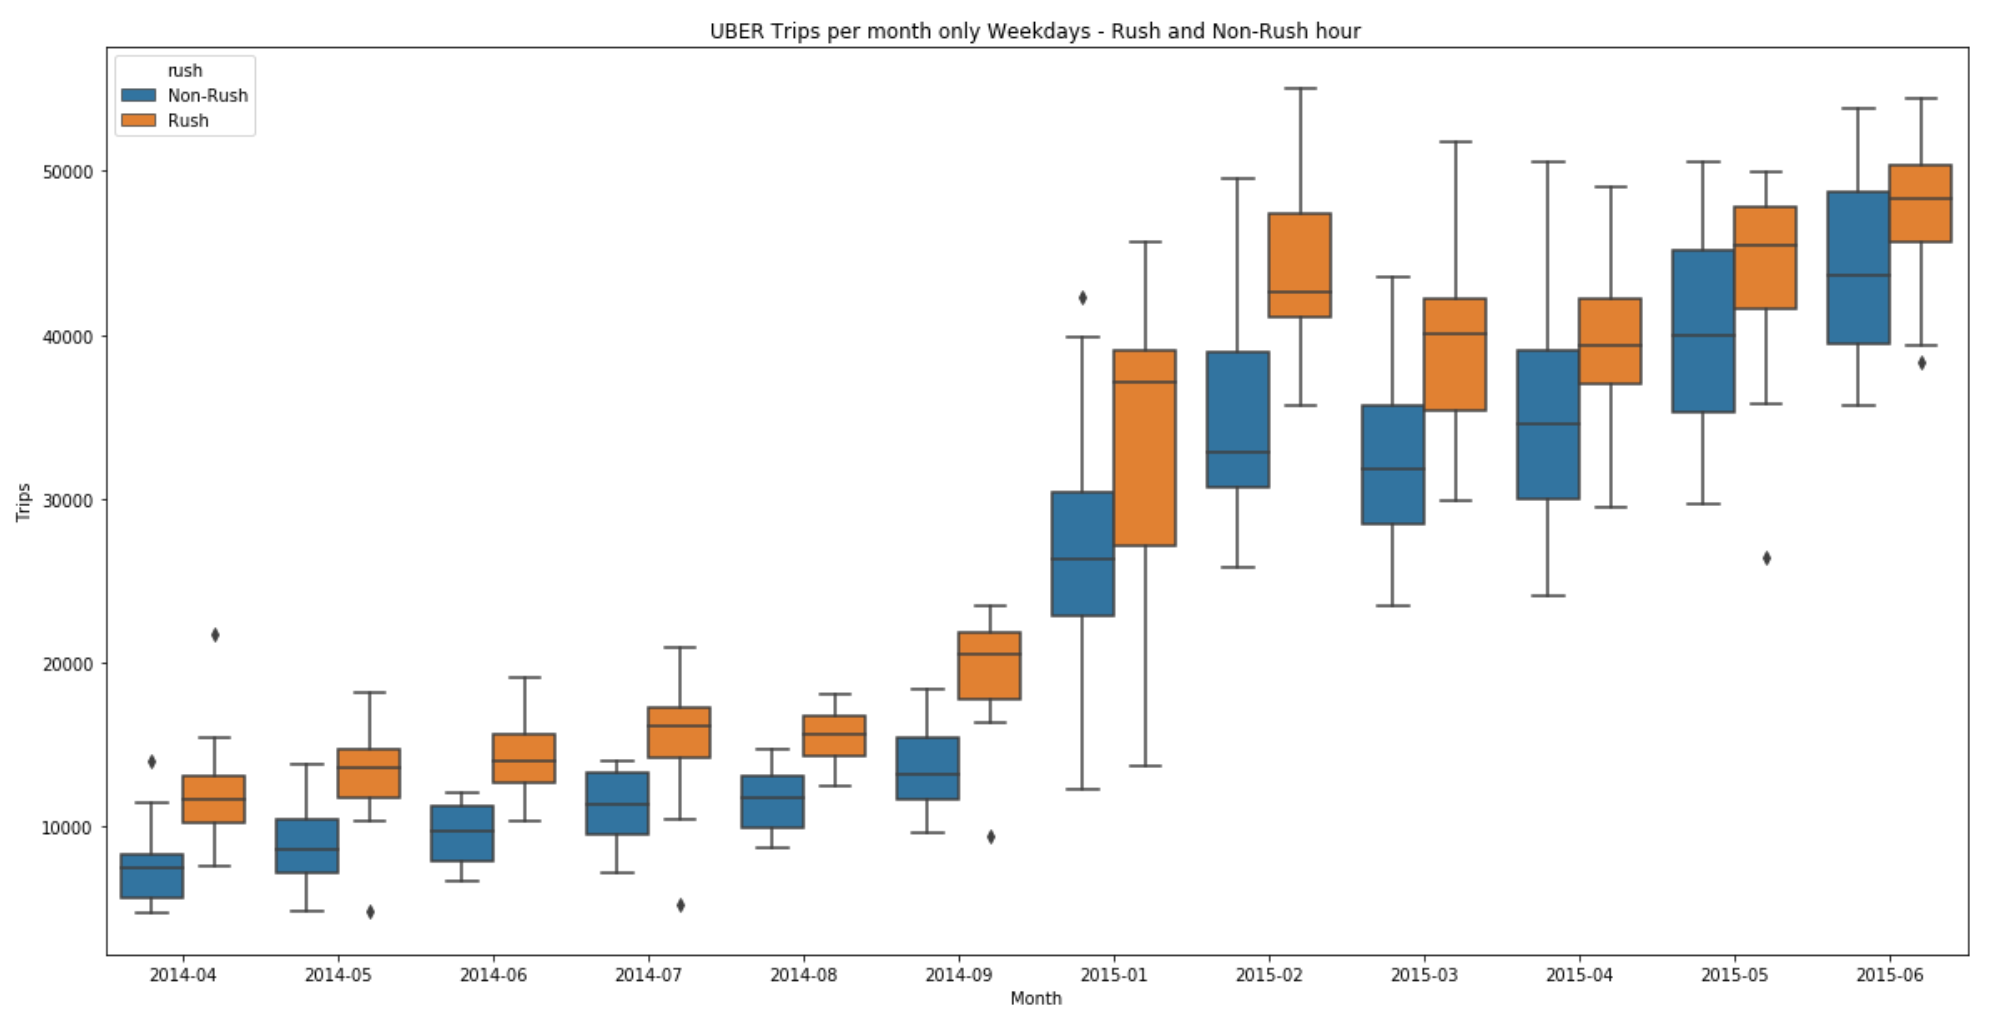
\includegraphics[height=2in, width=3.5in]{UBER_trips_only_weekdays_rush_and_non_rush.png}}%
\qquad
\subfigure[Yellow cab trips]{%
\label{fig:b}%
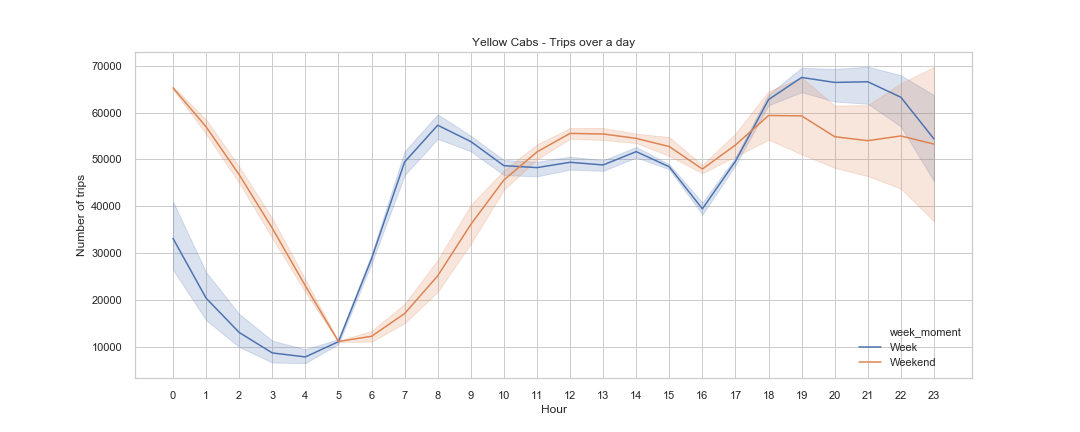
\includegraphics[height=2in, width=3.5in]{yellow_trips_hour_week.png}}%
\qquad
\subfigure[Green cab trips]{%
\label{fig:c}%
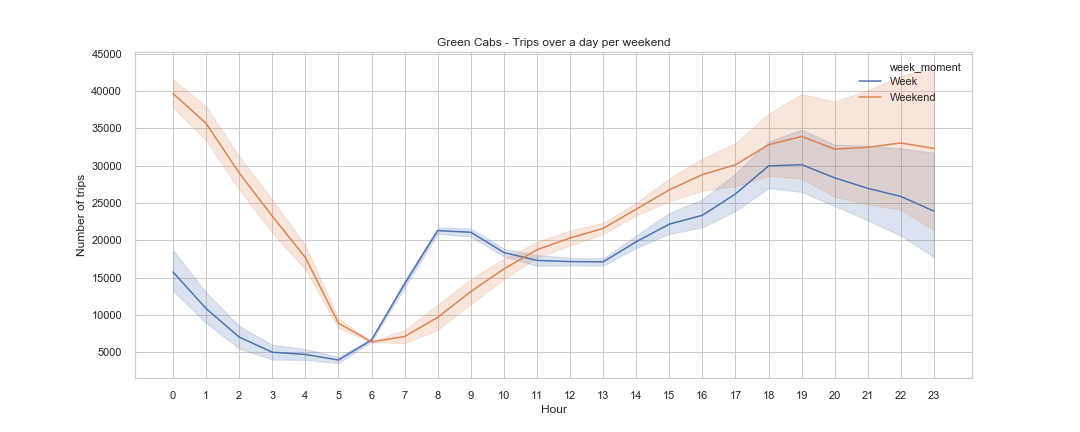
\includegraphics[height=2.4in, width=3.5in]{green_trips_hour_week.png}}%
\qquad
\subfigure[MTA trips]{%
\label{fig:d}%
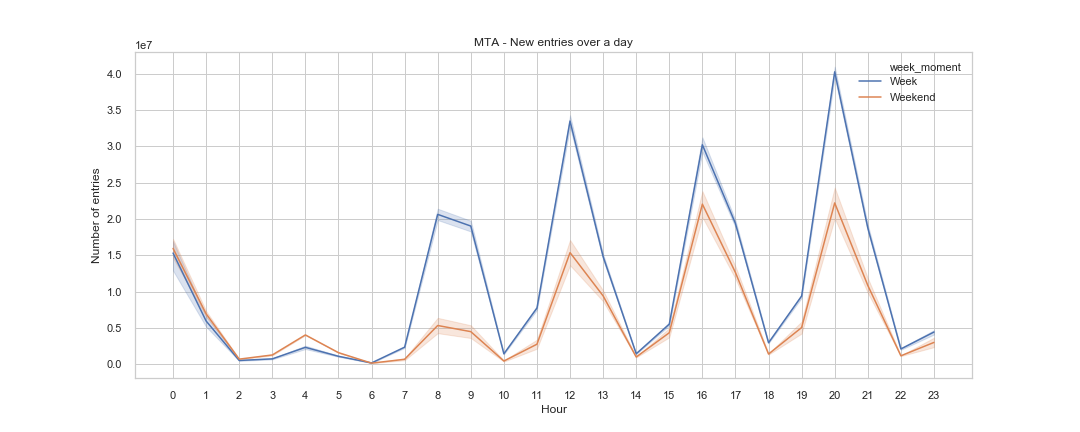
\includegraphics[height=2in, width=3.5in]{mta_entries_hour_week.png}}%
\caption{Hour week }
\label{fig:boxTrips}%
\end{figure}




\begin{figure}%
\centering
\subfigure[Uber trips.]{%
\label{fig:a}%
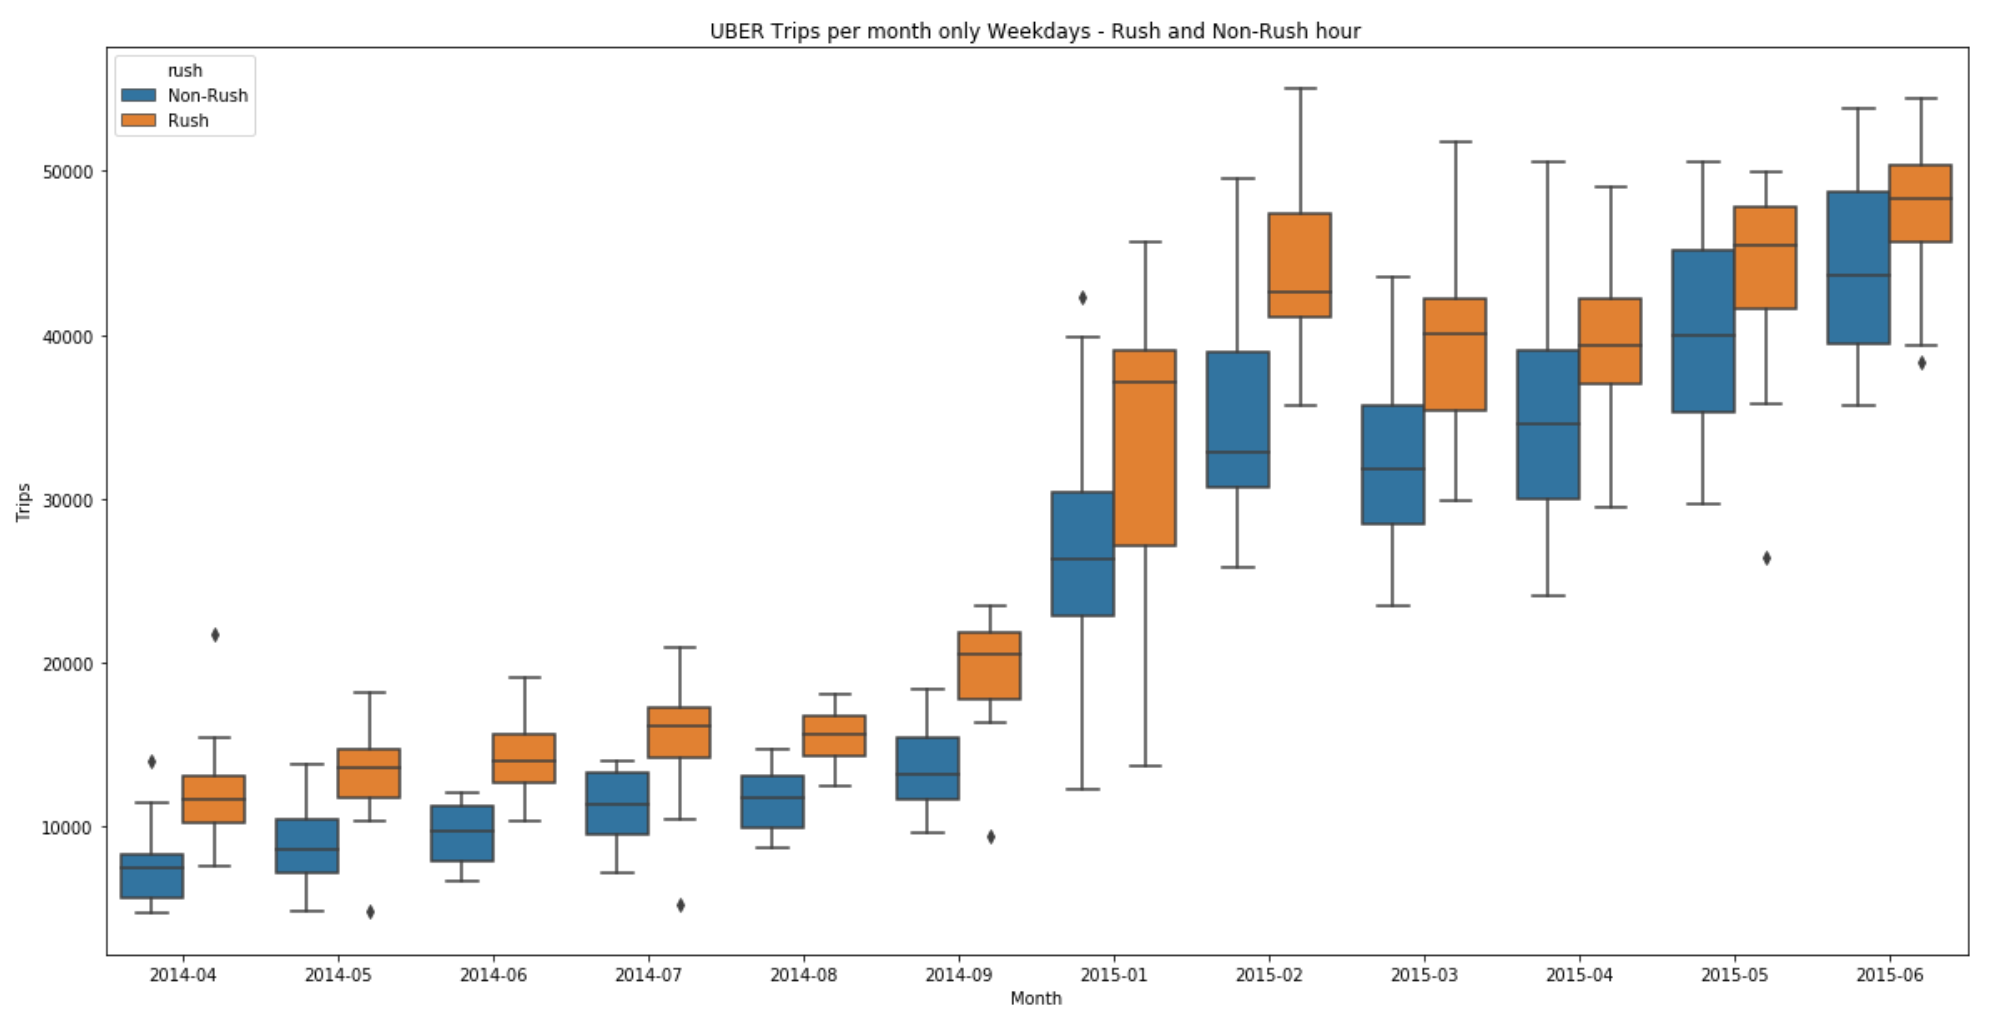
\includegraphics[height=2in, width=3.5in]{UBER_trips_only_weekdays_rush_and_non_rush.png}}%
\qquad
\subfigure[Yellow cab trips]{%
\label{fig:b}%
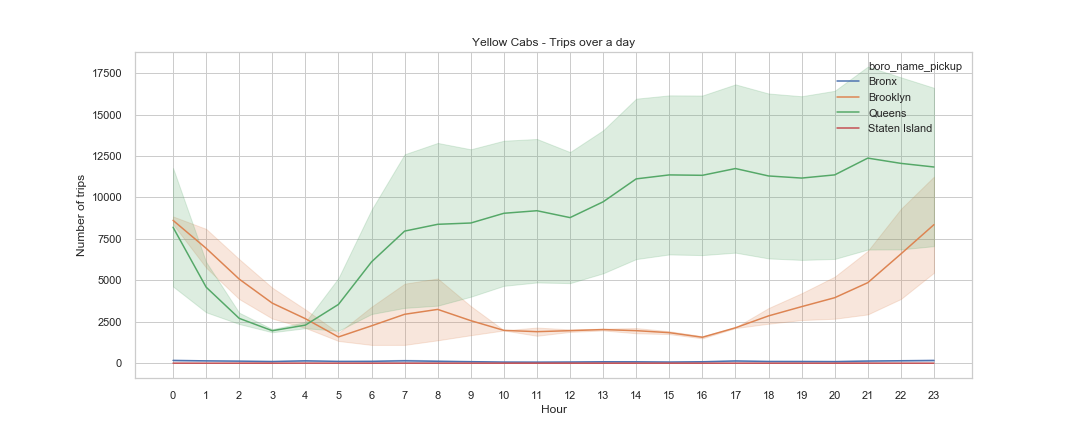
\includegraphics[height=2in, width=3.5in]{yellow_trips_hour_borough.png}}%
\qquad
\subfigure[Green cab trips]{%
\label{fig:c}%
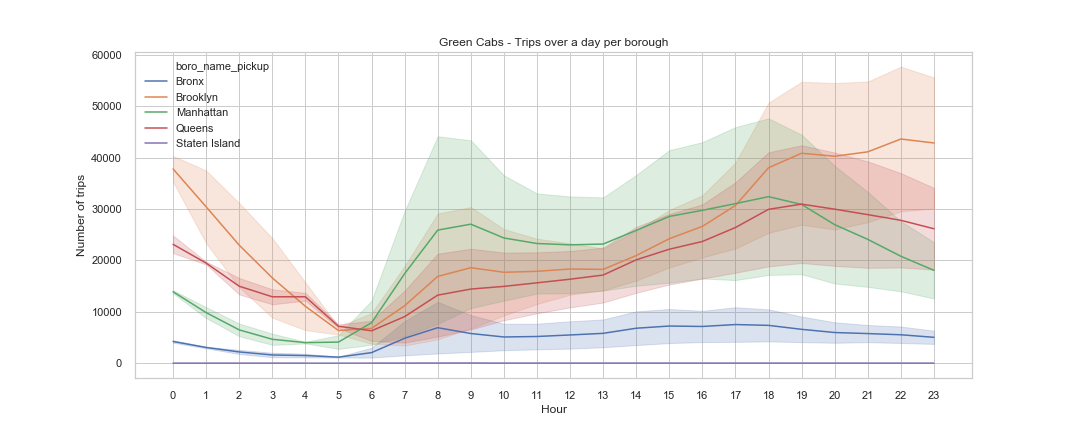
\includegraphics[height=2.4in, width=3.5in]{green_trips_hour_borough.png}}%
\qquad
\subfigure[MTA trips]{%
\label{fig:d}%
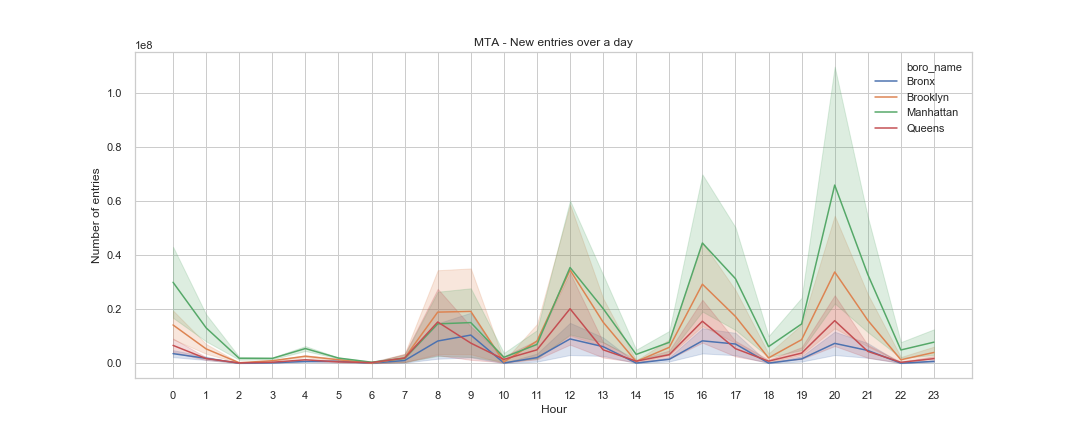
\includegraphics[height=2in, width=3.5in]{mta_entries_hour_borough.png}}%
\caption{Hour borough }
\label{fig:boxTrips}%
\end{figure}




\begin{figure}%
\centering
\subfigure[Uber trips.]{%
\label{fig:a}%
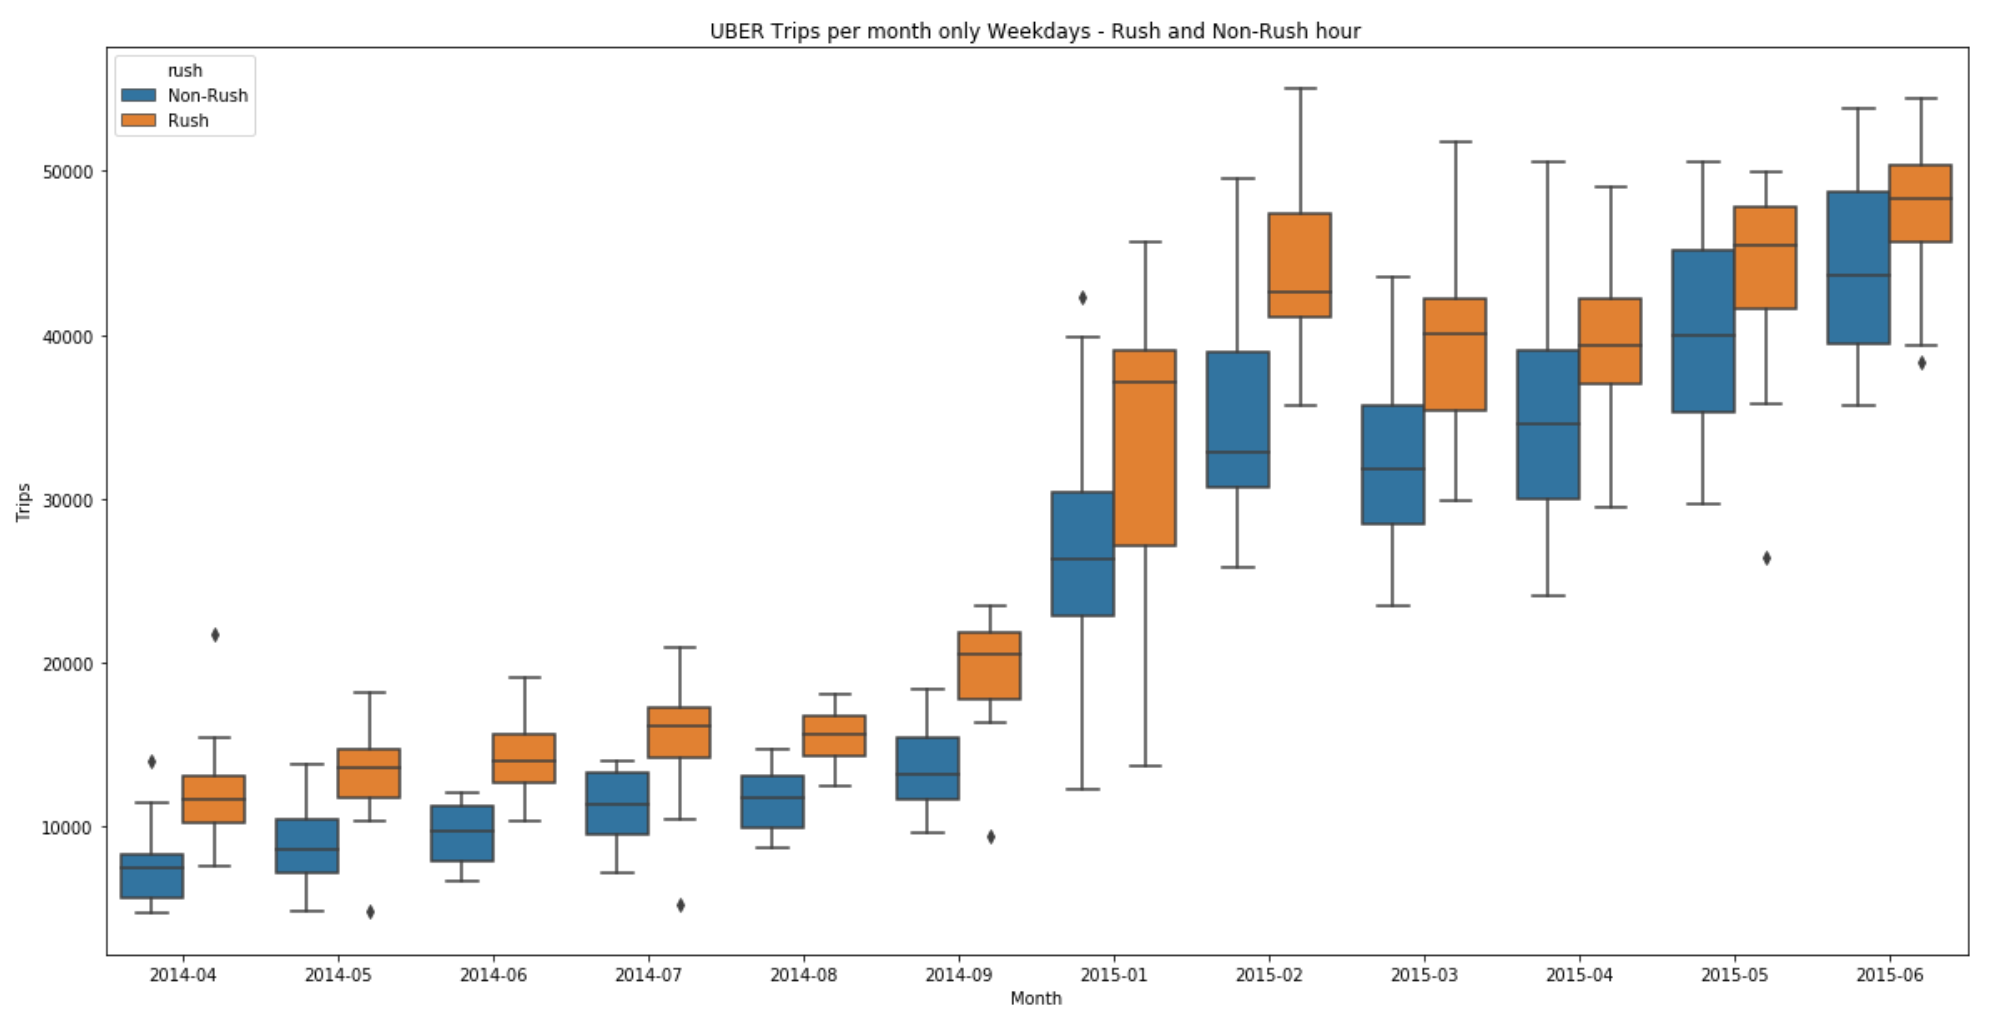
\includegraphics[height=2in, width=4in]{UBER_trips_only_weekdays_rush_and_non_rush.png}}%
\qquad
\subfigure[Yellow cab trips]{%
\label{fig:b}%
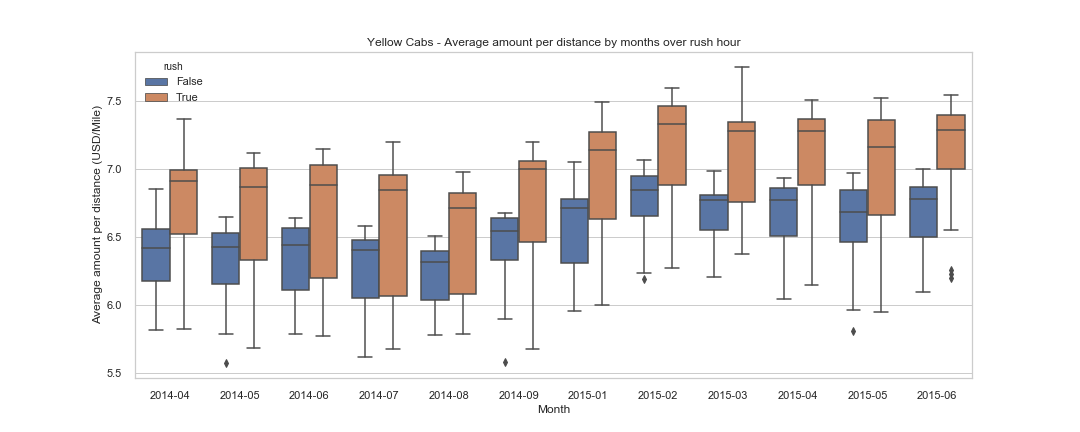
\includegraphics[height=2in, width=4in]{yellow_avgamountperdistance_rush_month_boxplot.png}}
\qquad
\subfigure[Green cab trips]{%
\label{fig:c}%
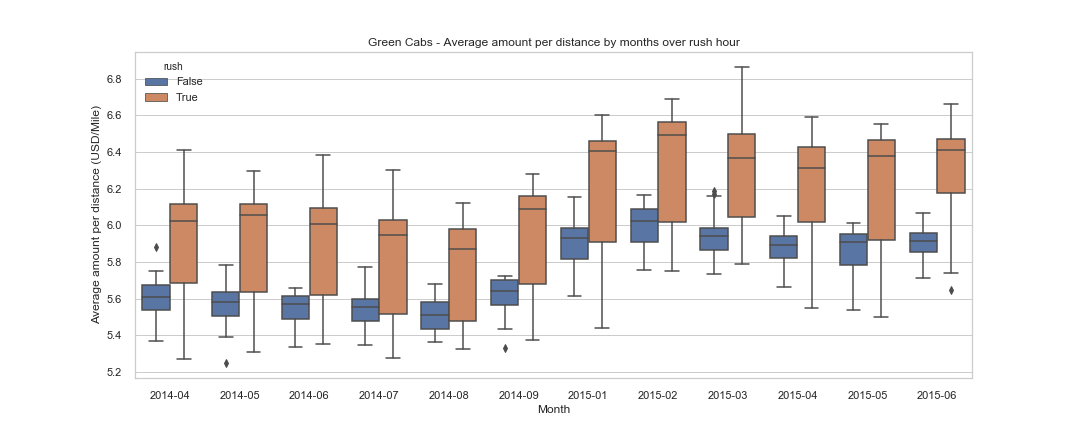
\includegraphics[height=2.4in, width=4in] {green_avgamountperdistance_rush_month_boxplot.png}}%
\caption{price per distance }
\label{fig:boxTrips}%
\end{figure}


\begin{figure}%
\centering
\subfigure[Uber trips.]{%
\label{fig:a}%
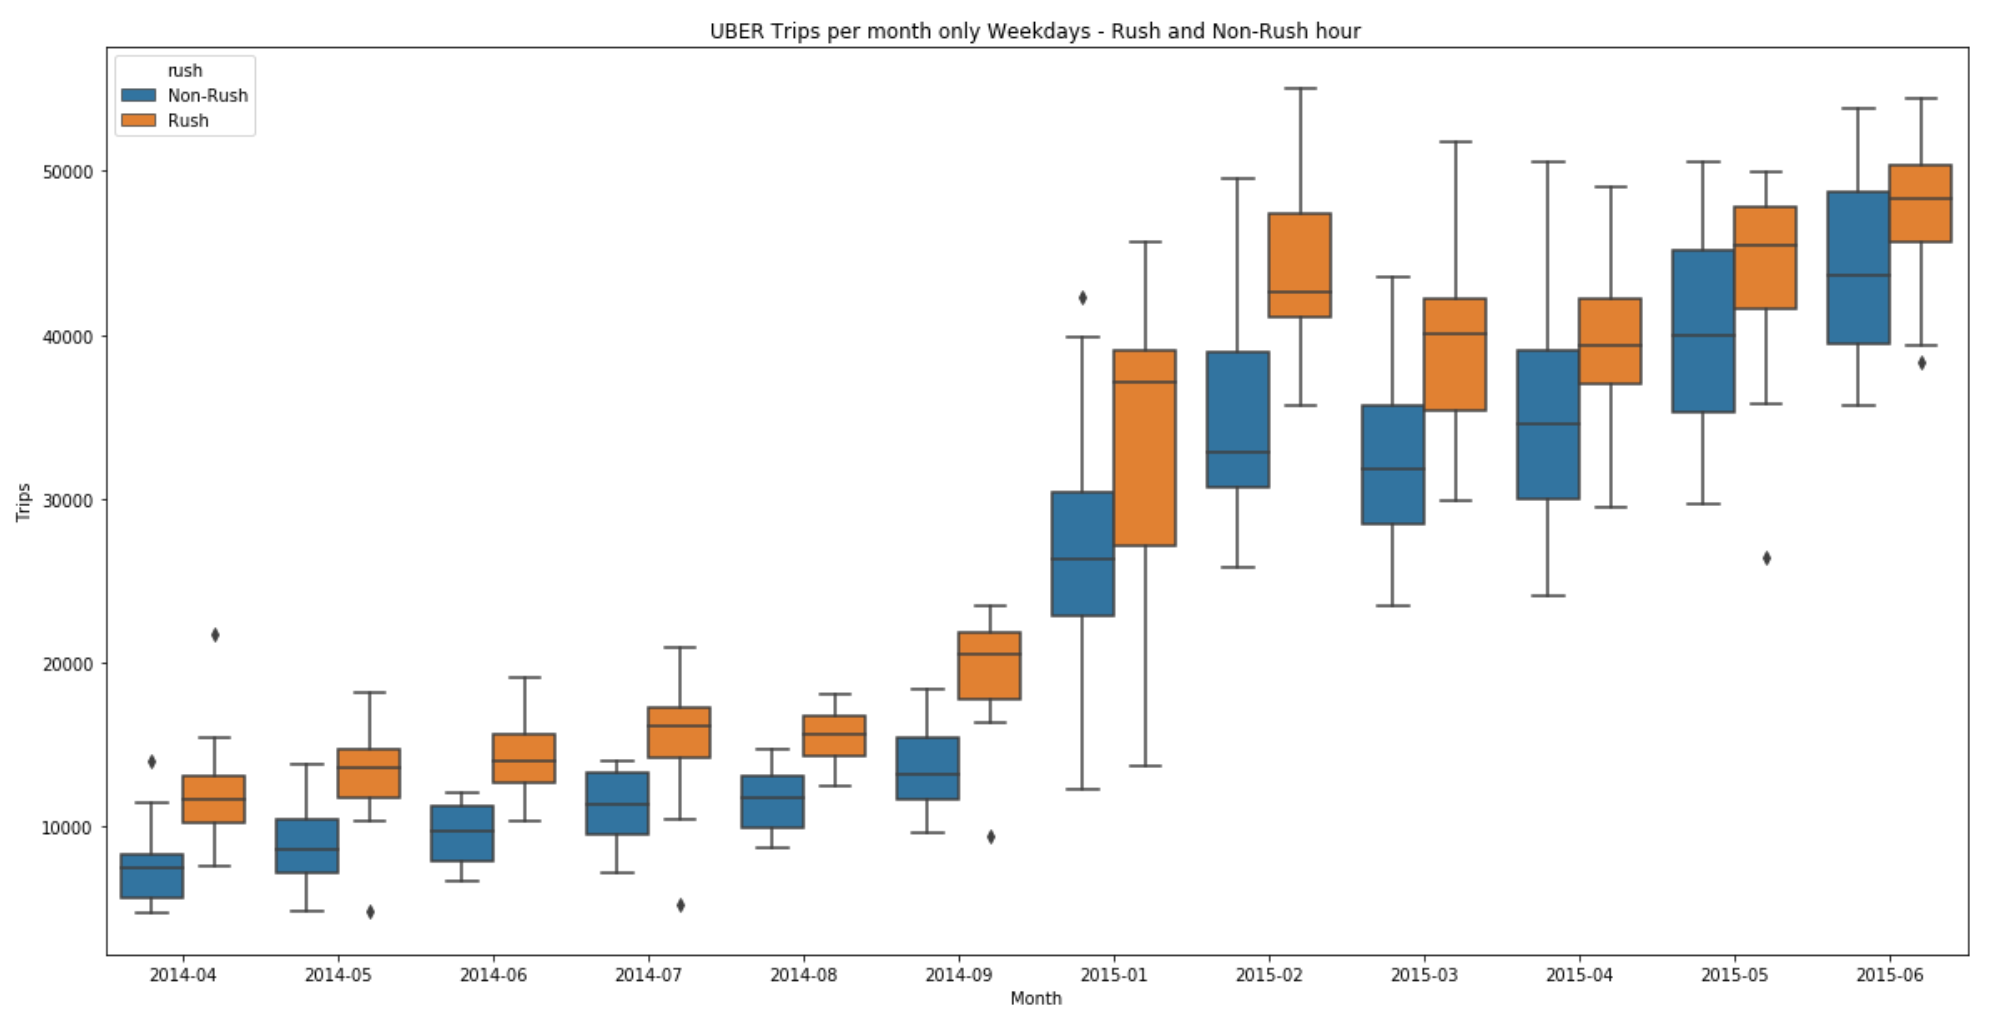
\includegraphics[height=2in, width=4in]{UBER_trips_only_weekdays_rush_and_non_rush.png}}%
\qquad
\subfigure[Yellow cab trips]{%
\label{fig:b}%
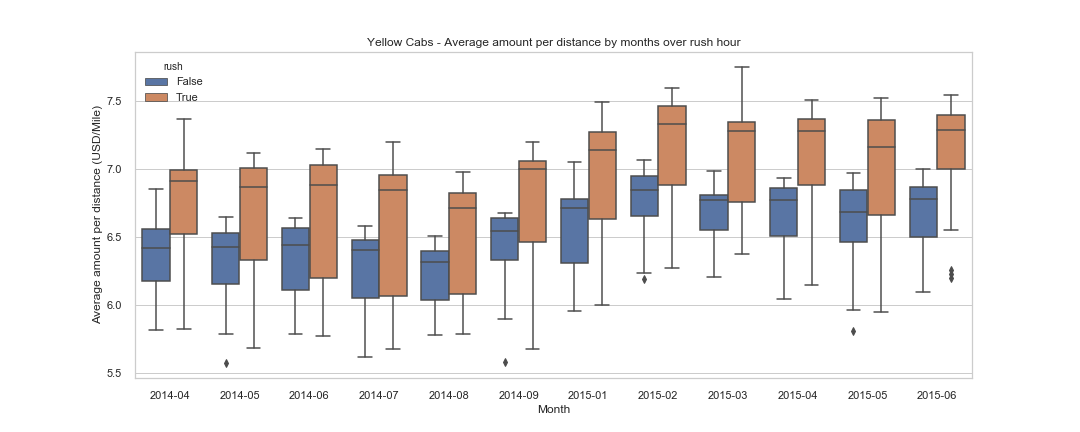
\includegraphics[height=2in, width=4in]{yellow_avgamountperdistance_rush_month_boxplot.png}}
\qquad
\subfigure[Green cab trips]{%
\label{fig:c}%
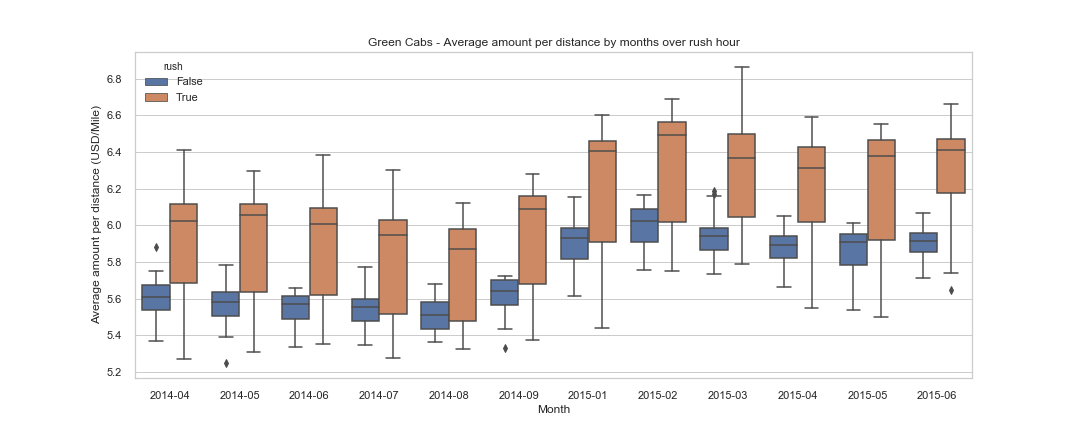
\includegraphics[height=2.4in, width=4in] {green_avgamountperdistance_rush_month_boxplot.png}}%
\caption{avrg distance }
\label{fig:boxTrips}%
\end{figure}



